\chapter{Analysis and Design}
\label{chapter:analysis.design}

Warlock is a distributed consensus service custom made to be used as a
lock manger. In this chapter, we discuss the design of the system based on the
requirements detailed in \chapterref{requirements}. We explain the structure
of the system and then detail how it maps on to the specified requirements.

\section{Architecture}

The goal for Warlock is to

\begin{itemize}
  \item Satisfy all the requirements specified in \chapterref{requirements}.
  \item Implement the system in Erlang while following OTP principles.
  \item Create a modular design to allow for customization for other projects.
\end{itemize}

The Warlock system can be divided into different components based on their
functionality as shown in figure \figureref{warlock.arch}. In terms of the
data flow and interaction between the components, the system design is quite
close to that of Chubby locks \citep{Burrows06} as in
\figureref{chubby.structure}.

\begin{figure}
  \begin{whole}
  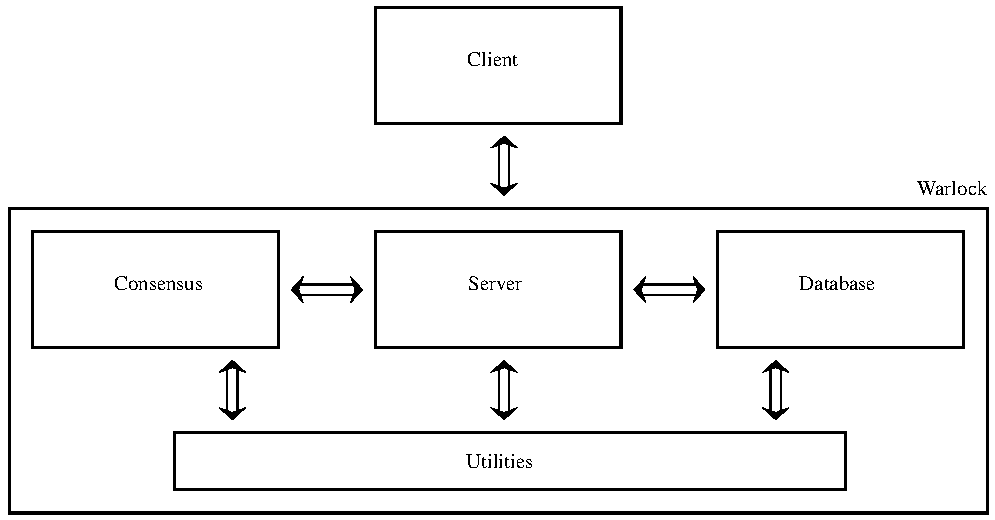
\includegraphics[width=\wholewidth]{warlock-architecture}
  \caption[Warlock Architecture]{%
    The figure shows the high level view of Warlock with its components and the
    messaging/dependencies between them.}
    \label{figure:warlock.arch}
  \normalcaption
  \end{whole}
\end{figure}

The figure shows the internal components of Warlock and the dependencies between
them.

With the design goal of keeping the system modular, we separate logically 
distinct parts of the system into Erlang applications \sectionref{concepts.otp}.
These applications interact with each other by function calls if they are 
libraries or by messaging if they are distinct processes. Below we detail the
purpose and functionality of each of these applications.

\subsection{Utilities}

The utilities component provides the rest of the Warlock components with
commonly used modules. The library consists of

\begin{itemize}
    \iterm{Configuration Helper}: Reads configuration files to be used as
    settings for Warlock.
    \iterm{Hash Table}: A hash table implementation based on ETS%
    \sidenote[-8]{
      Erlang Term Storage (ETS) is a an in-memory storage provided by the Erlang
      Virtual Machine. It supports multiple data structures and operations over
      them.}
    and dict%
    \sidenote[-3]{
      dict is Erlang's in-built dictionary implementation. Unlike ETS, it is
      immutable.}
\end{itemize}

It is used as a dependency in rest of the Warlock components. It also defines
Erlang macros%
\sidenote[5]{
  Erlang macros are similar to C macros. They allow us to define small functions
  and constants that is taken care of by the preprocessor during code
  compilation.
}
for enabling different levels of logging.

\subsection{Server}

The server component of Warlock ties all the other components together and
indirectly routes messages between them. It provides many functionality.

\subsubsection{Handle client connections}
\label{section:a.n.d.client.conn}

The system can be interacted with by

\begin{itemize}
  \item Embedding Warlock in the same virtual machine as the
    client application.
  \item Accessing the system using RPC.
  \item Using a well defined binary protocol.
\end{itemize}

The first two of the options are trivial to implement. For the last option, the
server manages the incoming client connections which can then send requests. The
client connections are over TCP and use the Redis binary protocol
\citep{RedisProtocol}%
\sidenote{
  The reasoning behind using the Redis binary protocol is that it is well
  defined and has a good set of features. It is also implemented in
  multiple languages allowing for usage from a much wider audience.
}. Once a connection is setup, it becomes an individual process unaffected by
other connections making it more robust.

\subsubsection{Callback}

Server provides the callback module that is executed once the request is
processed. This allows us to keep the core of Warlock independent of the
database implementation and to treat the commands as simple messages. This
helps increase the robustness of the consensus component by isolating the
command execution to the database component.

To enable replication \sectionref{analysis.design.replication} the
callback module needs to provide few additional features. The database
component of Warlock has to be in read-only mode to avoid the chances of
data corruption when it is a source node being replicated from. To allow
this, callback has two modes of operation.

\begin{itemize}
    \iterm{Active}: The callback module works normally accepting requests
    and forwarding them to the database component.

    Change from active to passive mode can be done immediately.
    \iterm{Passive}: The callback module add new decisions to a queue.

    When changing from passive to active mode, the queue is first processed
    asynchronously and mode change only happens when the queue is empty.
\end{itemize}

\subsubsection{Console}

Server provides interface that allows us to interact with Warlock from the
console. This allows us to start, setup and modify the Warlock cluster from
the command line. Command line access helps us use automation tools such as
Chef \citep{Chef} to rapidly deploy it on cloud servers
\citep{Armbrust:2010:VCC:1721654.1721672, amazonAWS}.

\subsubsection{Replication}
\label{section:analysis.design.replication}

For the requirement \sectionref{req.dynamic.cluster} of enabling a dynamic
cluster we need to enable to copy/replicate data between servers.
Server setups connection between two servers and oversees the data transfer
between them when a new node is being added to the cluster. The steps for
this are:

\begin{itemize}
  \item All the nodes in the member group listen on a predefined port.
  \item A command is executed on the new node that is to be added to the cluster
    with the address of a seed%
    \sidenote{
      A \emph{seed node} in this context is one that provided all the necessary
      information to setup a data transfer connection.
    } node.
  \item The seed node sends the target node (new node) with the information of
    the source node%
    \sidenote[1]{
      Since data transfer is resource intensive, we do not use the master node
      as the seed. So the \emph{source node} is picked to be a health cluster
      member other than the master.
    }.
  \item The target node sets up a TCP connection with the seed node and sends
    a SYNC%
    \sidenote[3]{
      The \emph{SYNC} signal is used to indicate that the target node is ready
      to receive the data.
    } signal.
  \item On the reception of the signal, the seed node does the following:
    \begin{itemize}
      \item Change the status of the callback module to ``passive''.
      \item Ask the database component to backup the entire database to a
        predefined file.
      \item Transfer the file to the target node using a binary protocol.
      \item Once transfer is complete and the callback module has synced
        the data of the two nodes, request for a state reconfiguration via
        consensus.
      \item Once callback queue is processes, reset it back to ``active'' state.
    \end{itemize}
  \item On the reception of the data file, the target machine does the
    following:
    \begin{itemize}
      \item Reset the local database.
      \item Load the transferred file into the database.
      \item Receive commands from the source node when it executes its local
        command queue.
      \item Gets added to the members group and closes connection with the
        source node.
    \end{itemize}
\end{itemize}

\subsection{Database}

The database component is used to store all the data and provides at its
least the simple API required for a key value store.

\subsubsection{Pluggable back ends}

As per the requirement \sectionref{ml.kv.store}, the database needs to a
key value store. However, any type of database can be used
since Warlock by itself does not execute the commands. The commands are passed
on to the database driver after a successful round allowing us the flexibility
to use other types of databases. We create a specific behaviour%
\sidenote{
  Erlang behaviours \citep{ErlangBehaviour} are a set of specifications that
  can be used to create a generic reusable component.
}
for this purpose. Drivers can then be written for different databases
implementing the functions specified in the behaviour.

\subsubsection{Key Expiry}
\label{section:a.n.d.expiry}

Allowing stored objects to expire after a certain period of time allows the
system to remove entries which were left behind when the cleanup process
of the application using the system fails. However, key expiry in is a
complex process in itself \todo{appendix?} which can potentially lead to
poor performance. For our system, we store the expiry time, but cleanup is
only done when it gets accessed the next time. This allows us to keep
flexibility while keeping the system performance predictable.

Besides the simple database interface, the this component can provide data
backup and restore functions that can be used by the server component to
enable the Warlock feature of adding fresh nodes dynamically.

\subsection{Consensus}

The consensus component is the core of Warlock. It uses a modified version of
the Paxos algorithm from \citet{Robbert2011} as described in
\chapterref{concepts} for its implementation. It also
uses ideas from \citet{LamportSP08} and \citet{LamportMZ10} to allow for
a dynamic cluster. However, the algorithm needs some modifications
\sectionref{consensus.optimization} before it can be used.

\section{Reconfigurable State Machine}
\label{section:a.n.d.reconfig}

The set of valid nodes in the cluster that take part in the protocol must
be static. We need to explicitly design the system to handle the requirement
\sectionref{req.dynamic.cluster}. This can be done by following certain
ideas from \citet{LamportSP08} and \citet{LamportMZ10}.

We can achieve this by treating the consensus state itself as a separate
parallel state machine along with the data state machine. Now we can use
the Paxos protocol itself to reconfigure the consensus state which consists
of the list of valid member nodes among other data. This modification allows
us to add new nodes, remove existing nodes, replace nodes as required at any
point of time.

For the implementation, instead of using the regular slots, we use specialized
alphabetic indexes allowing us better control during reconfiguration. This also
allows us to make the reconfiguration immediately instead of blocking requests
like in \citet{LamportSP08}.

The ballot is made up the leaders unique id and a monotonically increasing
integer that increments whenever there is a change in the leader. It is possible
that messages tagged with the old ballot is still in transit after a
reconfiguration. We introduce a new variable called ``view'' to avoid conflicts
caused by this. ``view'' is a monotonically increasing integer that increments
whenever there is a cluster configuration change

The downside of this specific design is that if the master changes during
reconfiguration, any of the proposals making progress will time out. It
should be possible to fix this by transferring such proposals to the new master
as new proposals.

\section{Consensus Optimization}
\label{section:consensus.optimization}

The straight implementation of Paxos is not very efficient owing to the overhead
that comes with duplicate messages, duplicate states and the detection of these
duplicates. The default implementation also requires the entire history of the
state be stored making it impractical. This section describes the optimizations
performed in this project, some of which are from \citet{Robbert2011}.

\subsection{Backoff and Preemption}

Consider the following situation in a Paxos system with two leaders L1 and L2.

\begin{itemize}
  \item L1 initiates the protocol by issuing P1a message.
  \item L1 receives quorum acceptance and all the acceptors accept its ballot.
  \item L2 initiates the protocol by issuing P1a message.
  \item L2 receives quorum acceptance and all the acceptors accept its ballot.
  \item L1 initiates P2a phase only to be preempted with a higher ballot.
  \item L1 initiates phase 1 with a P1a message.
  \item L2 initiates P2a phase only to be preempted with a higher ballot.
\end{itemize}

As we can see, this leads to a race condition which can exist indefinitely. To
fix this, whenever a leader is preempted, it waits for a predefined period of
time called the ``backoff'' time. This provides the leader with the higher
ballot sufficient time to make progress, thus avoiding the deadlock.

\subsection{Timeouts}

The leaders launches scouts and commanders depending on the phase the protocol
is currently running in. These processes have to wait for the response from
a quorum of acceptors after sending out their initial message. It is possible
that not all of these acceptors respond due to reasons such as a network
partition%
\sidenote{
  \emph{Network Partition}; In a connected group of nodes, the connection
  between the nodes can be severed in such a way that it creates two separate
  smaller groups termed ``partitions''.
}.

Introduction of timeouts in scouts and commanders allows us to timebox the
protocol creating a maximum bound for response time to the client. The client
itself can use timeouts, but this should always be greater than the internal
Warlock timeout to maintain consistency.

\subsection{State reduction}

In the basic version of Paxos, the acceptor maintains all the accepted values
for all the slots. This can be reduced by having the acceptor store only the
value corresponding to the maximum ballot for each slot resulting in smaller
acceptor state and P1b message size sent to the leader.

The acceptors are notified at the end of a successful operation. This allows
the them to store the values for only the slots that are currently making
progress resulting in reduced P1b message size.

Similarly the replica only needs to maintain the data for slots that are
making progress allowing it to purge data for decided slots. The leader can
also purge the completed proposal data it maintains to spawn commanders.

All the above optimizations are possible by co-locating replica, leader
and acceptor for each node. While it is possible to use shared data structures
between these processes residing on the same node, we avoid it to allow for
a cleaner implementation.

\subsection{Master Node and Leases}
\label{section:a.n.d.lease}

A leader that is not preempted can proceed directly with phase 2 of the
protocol for a proposal cutting the message latency by half. We use the
mechanism of lease to use this to our advantage.

The initial node whose leader manages to complete one round of Paxos is
termed the master node. We define a period of time called the master lease
during which leaders from other nodes cannot spawn scouts to push for a
higher ballot. The master renews its lease before it expires.

Failure detectors%
\sidenote{
  Erlang has built in failure detectors called monitors \citep{ErlangMonitor}.
  Using this feature it is possible to monitor the failure of local or
  remote processes.
}
are used to detect if the master node goes down to accelerate the election
of the next master node. The leaders from other node themselves try to
get election as soon as the lease of the current master expires. If the
failure detector takes a long time, then the system as a whole
stops making progress as long as the lease lasts. By balancing the lease
time, we can restrict the system to have reasonably short down times in
the worst case.

Usage of lease introduces a timing requirement into the system. The system
assumes that there is a definite bound on clock drift%
\sidenote{
  \emph{Clock drift}: Due to physical and mechanical limitations in building
  clocks, the time maintained by individual clocks tend to drift away from
  each other. Many mechanisms can be used to correct the drift, allowing us to
  set a bound on this drift.
} 
between the nodes.

\subsection{Message Reduction}

\chapterref{concepts} discussed the Paxos protocol used detailing the number
of messages sent between processes. By co-locating sets of processes and
using a master node, we can reduce this number by a large extent.

In the reduced version, the client sends the message directly to the
replica on the master node (master replica). The master replica only
sends the proposal to the local leader (master leader). On receiving quorum
acceptance, the leader directly responds to the client.

The above optimization allows us reduce the number of messages from
$O(n^2)$ to $O(n)$.

\subsection{Monitoring}

All the member nodes%
\sidenote{
  \emph{Member nodes}: Nodes which are in sync with rest of the cluster
and actively take part in the consensus protocol.}
keep a list of available nodes.
The leader of the master node monitors the leaders of rest of the member
of the cluster. When the master leader detects any failures, it moves the
node from the list of available nodes to the list of down nodes via the
consensus protocol.

Failure of the master leader itself will eventually trigger the election
leading to a new master node. This node will then take over the role of
monitoring rest of the members.

\section{API Design}

We try and keep the Application Programming Interface (API) of Warlock as
simple as possible. A typical command is of the format
\sourcecoderef{warlock.generic.cmd}

\begin{scode}{Erlang}{warlock.generic.cmd}{%
  Warlock's generic command format}{%
  Warlock's generic command format}
  \begin{lstlisting}
war_server:x(<location>, <command>)
  \end{lstlisting}
\end{scode}

The parts of the format are:

\begin{itemize}
  \item \texttt{war\_server:x} is the module and function name which acts
    as the external interface.
  \item \texttt{<command>} operation requested by the client that has to
    be eventually executed by the database component.
  \item \texttt{<location>} indicates where \texttt{<command>} has to be
    run.
\end{itemize}

\begin{scode}{Erlang}{warlock.clu.cmd}{%
  Warlock's cluster command format}{%
  Warlock's cluster command format}
  \begin{lstlisting}
1> (warlock@127.0.0.1)> war_server:x(clu, [set, key, value]).
{ok,success}
  \end{lstlisting}
\end{scode}


\begin{scode}{Erlang}{warlock.loc.cmd}{%
  Warlock's local command format}{%
  Warlock's local command format}
  \begin{lstlisting}
2> (warlock@127.0.0.1)> war_server:x(loc, [get, key]).
{ok,value}
  \end{lstlisting}
\end{scode}

\texttt{<location>} has two possible values:

\begin{itemize}
    \iterm{Cluster}: Cluster (\texttt{clu}) indicates that the full
    consensus protocol must be run so that the command can be executed
    on all the servers.

    The commands are run on \texttt{clu} whenever its execution changes
    the database's state. For example, \sourcecoderef{warlock.clu.cmd}

    \iterm{Local}: Local (\texttt{loc}) indicates that the command only
    needs to be run on the local replica the client is connected to.

    The commands that have no effect on the database's state can be run
    on \texttt{loc}. For example, \sourcecoderef{warlock.loc.cmd}
\end{itemize}


\section{Read Write separation}

As per the requirement \sectionref{req.read.write.ratio}, we need to design the
system to support read loads that are in multiple of the maximum possible write
loads. It also follows from the system design that each node (replica) has the
entire dataset available and that we do not need consensus to access it. 

Since the system is quorum based, not all of the nodes in the group take part
in every round of consensus. This means that there are possibilities of a few 
slow nodes existing in the system. Reading data directly from these nodes might
possibly get stale data.

The solution is to use a compromise between having fresh data and accepting 
chances slightly stale data in lieu for huge performance improvements. The
use of leases described in \sectionref{a.n.d.lease} allows us to minimize the
chances of stale data. The lease is renewed by the master node as per preset 
time (typically 5 seconds). We use this lease time at the individual node level 
to check if we are in sync with the rest of the nodes. This allows us to serve 
read-only data from individual nodes directly with a predictable limit on the 
age of data. In case the lease has expired, we return an error response to
the client in line with the goal of serving consistent data.

\section{Failure Recovery}

The system should be able to withstand problems such as node failures and data
corruption. This is a hard problem to solve in system with static configuration
since they have to implement complex error correction and conflict resolution
mechanisms. However, since we support dynamic configuration, we can replace
the problem node with a fresh node. Granular control allows us to detach the
problem nodes with the intention of debugging the error.

The current design supports resetting a node's data and replicating from
a member with good data. Improvements are possible in this area in terms of
performance and usage of less resources as discussed in
\chapterref{future.work}.







